\chapter{General-Purpose Microprocessors}\label{ch:gp}

\begin{objectives}
After studying this chapter you will be able to:
\begin{itemize}
  \item explain how a general-purpose processor differs from a dedicated one, and describe the instruction cycle (fetch, decode, execute);
  \item define an instruction set and its binary encoding;
  \item describe the datapath and control unit of the simple processors EC-1 and EC-2 and trace the execution of a program;
  \item explain why the control unit needs wait states when memory is synchronous;
  \item write, assemble and trace small programs in machine code, and load them into memory with an Intel HEX file; and
  \item describe how the step from ROM to RAM leads to the von Neumann stored-program computer.
\end{itemize}
\end{objectives}

\section{General-Purpose Microprocessors}
The dedicated processors of \cref{ch:dedicated} perform one task, wired into their structure. A \term{general-purpose microprocessor} can perform many different functions: its function is determined by the \emph{instructions} it executes, which are stored in memory as a \term{program}. Changing the program changes the function without changing the hardware. The Intel Core and ARM Cortex processors are examples.

\begin{keypoint}[A processor is a dedicated processor]
A general-purpose processor can be viewed as a \emph{dedicated} processor whose single task is to \textbf{fetch and execute instructions}. The ``data'' that it processes include the instructions themselves.
\end{keypoint}

We therefore design it with the methods of the previous chapter. The designs of this chapter, the 8-bit processors \textbf{EC-1} and \textbf{EC-2}, follow the educational processor designs of Hwang~\cite{hwang2005,hwang2018}; the structure, the VHDL descriptions, the programs and the simulations presented here are the author's implementations for this course.

\section{Overview of CPU Design}\label{sec:cpu-design}
Designing a central processing unit (CPU) has three steps.
\begin{enumerate}
  \item \textbf{Define the instruction set}: the operations the processor performs (add, load, jump, \dots) and how each instruction is encoded in binary (an \term{opcode} and its \term{operands}).
  \item \textbf{Design the datapath}: a datapath that can execute \emph{every} instruction of the set. It contains the \term{program counter} (PC), which holds the address of the next instruction; the \term{instruction register} (IR), which holds the current instruction; the ALU or other functional units; registers; and memory.
  \item \textbf{Design the control unit}: an FSM that executes the \term{instruction cycle}: \textbf{fetch} the instruction from memory (at the address in the PC) into the IR, \textbf{decode} it by examining the opcode, and \textbf{execute} it by issuing the control signals for the operation.
\end{enumerate}

\section{The EC-1 Microprocessor}\label{sec:ec1}
\subsection{Overview}
To keep the design small enough to do by hand, EC-1 is a simple 8-bit processor with:
\begin{itemize}
  \item an \textbf{8-bit} data width;
  \item a \textbf{4-bit} address, hence $2^4=16$ memory words;
  \item a \textbf{read-only memory} (ROM) that holds the program; and
  \item one data register, the \term{accumulator} $A$.
\end{itemize}
It is an \emph{accumulator machine}: every operation takes its operand from, and returns its result to, register $A$.

\subsection{Instruction set}
EC-1 has only five instructions. The opcode occupies the 3 most significant bits of the 8-bit instruction (\cref{tab:ec1-is}). Opcodes 000, 001 and 010 are unused (no operation); the bits shown as \texttt{x} are don't-cares and \texttt{aaaa} is a 4-bit address.

\begin{table}[htbp]
\centering
\caption{The EC-1 instruction set.}
\label{tab:ec1-is}
\begin{tabular}{llll}
\toprule
Mnemonic & Encoding & Operation & Description\\ \midrule
\texttt{IN A} & \texttt{011 xxxxx} & $A\leftarrow$ Input & input a byte into $A$\\
\texttt{OUT A} & \texttt{100 xxxxx} & Output $\leftarrow A$ & output $A$\\
\texttt{DEC A} & \texttt{101 xxxxx} & $A\leftarrow A-1$ & decrement $A$\\
\texttt{JNZ addr} & \texttt{110 xaaaa} & if $A\neq0$, $PC\leftarrow aaaa$ & jump if not zero\\
\texttt{HALT} & \texttt{111 xxxxx} & halt & stop execution\\ \bottomrule
\end{tabular}
\end{table}

\subsection{Datapath}
The datapath (\cref{fig:ec1-dp}) must support fetching instructions and executing them.
\begin{itemize}
  \item The \textbf{program counter} PC (4 bits) addresses the ROM. Normally $PC\leftarrow PC+1$ (the incrementer). For \texttt{JNZ} with $A\neq0$, $PC\leftarrow IR[3:0]$; the multiplexer \textit{JNZmux} chooses between the incremented PC and the jump address.
  \item The \textbf{instruction register} IR (8 bits) holds the instruction read from the ROM. Its top three bits $IR[7:5]$ are the opcode that goes to the control unit.
  \item The \textbf{accumulator} $A$ (8 bits) takes its input either from the external input port or from the decrementer ($A-1$); the multiplexer \textit{INmux} chooses ($1$ = Input, $0$ = Dec).
  \item A \textbf{zero detector} (an 8-input OR gate on $A$) generates the status signal $A\neq0$ for the control unit.
  \item A \textbf{three-state buffer} controlled by \textit{OutE} drives the output port with $A$.
\end{itemize}
The control signals, produced by the control unit, are \textit{IRload}, \textit{PCload}, \textit{INmux}, \textit{Aload}, \textit{JNZmux}, \textit{OutE} and \textit{Halt}.

\begin{sidewaysfigure}[p]
\centering
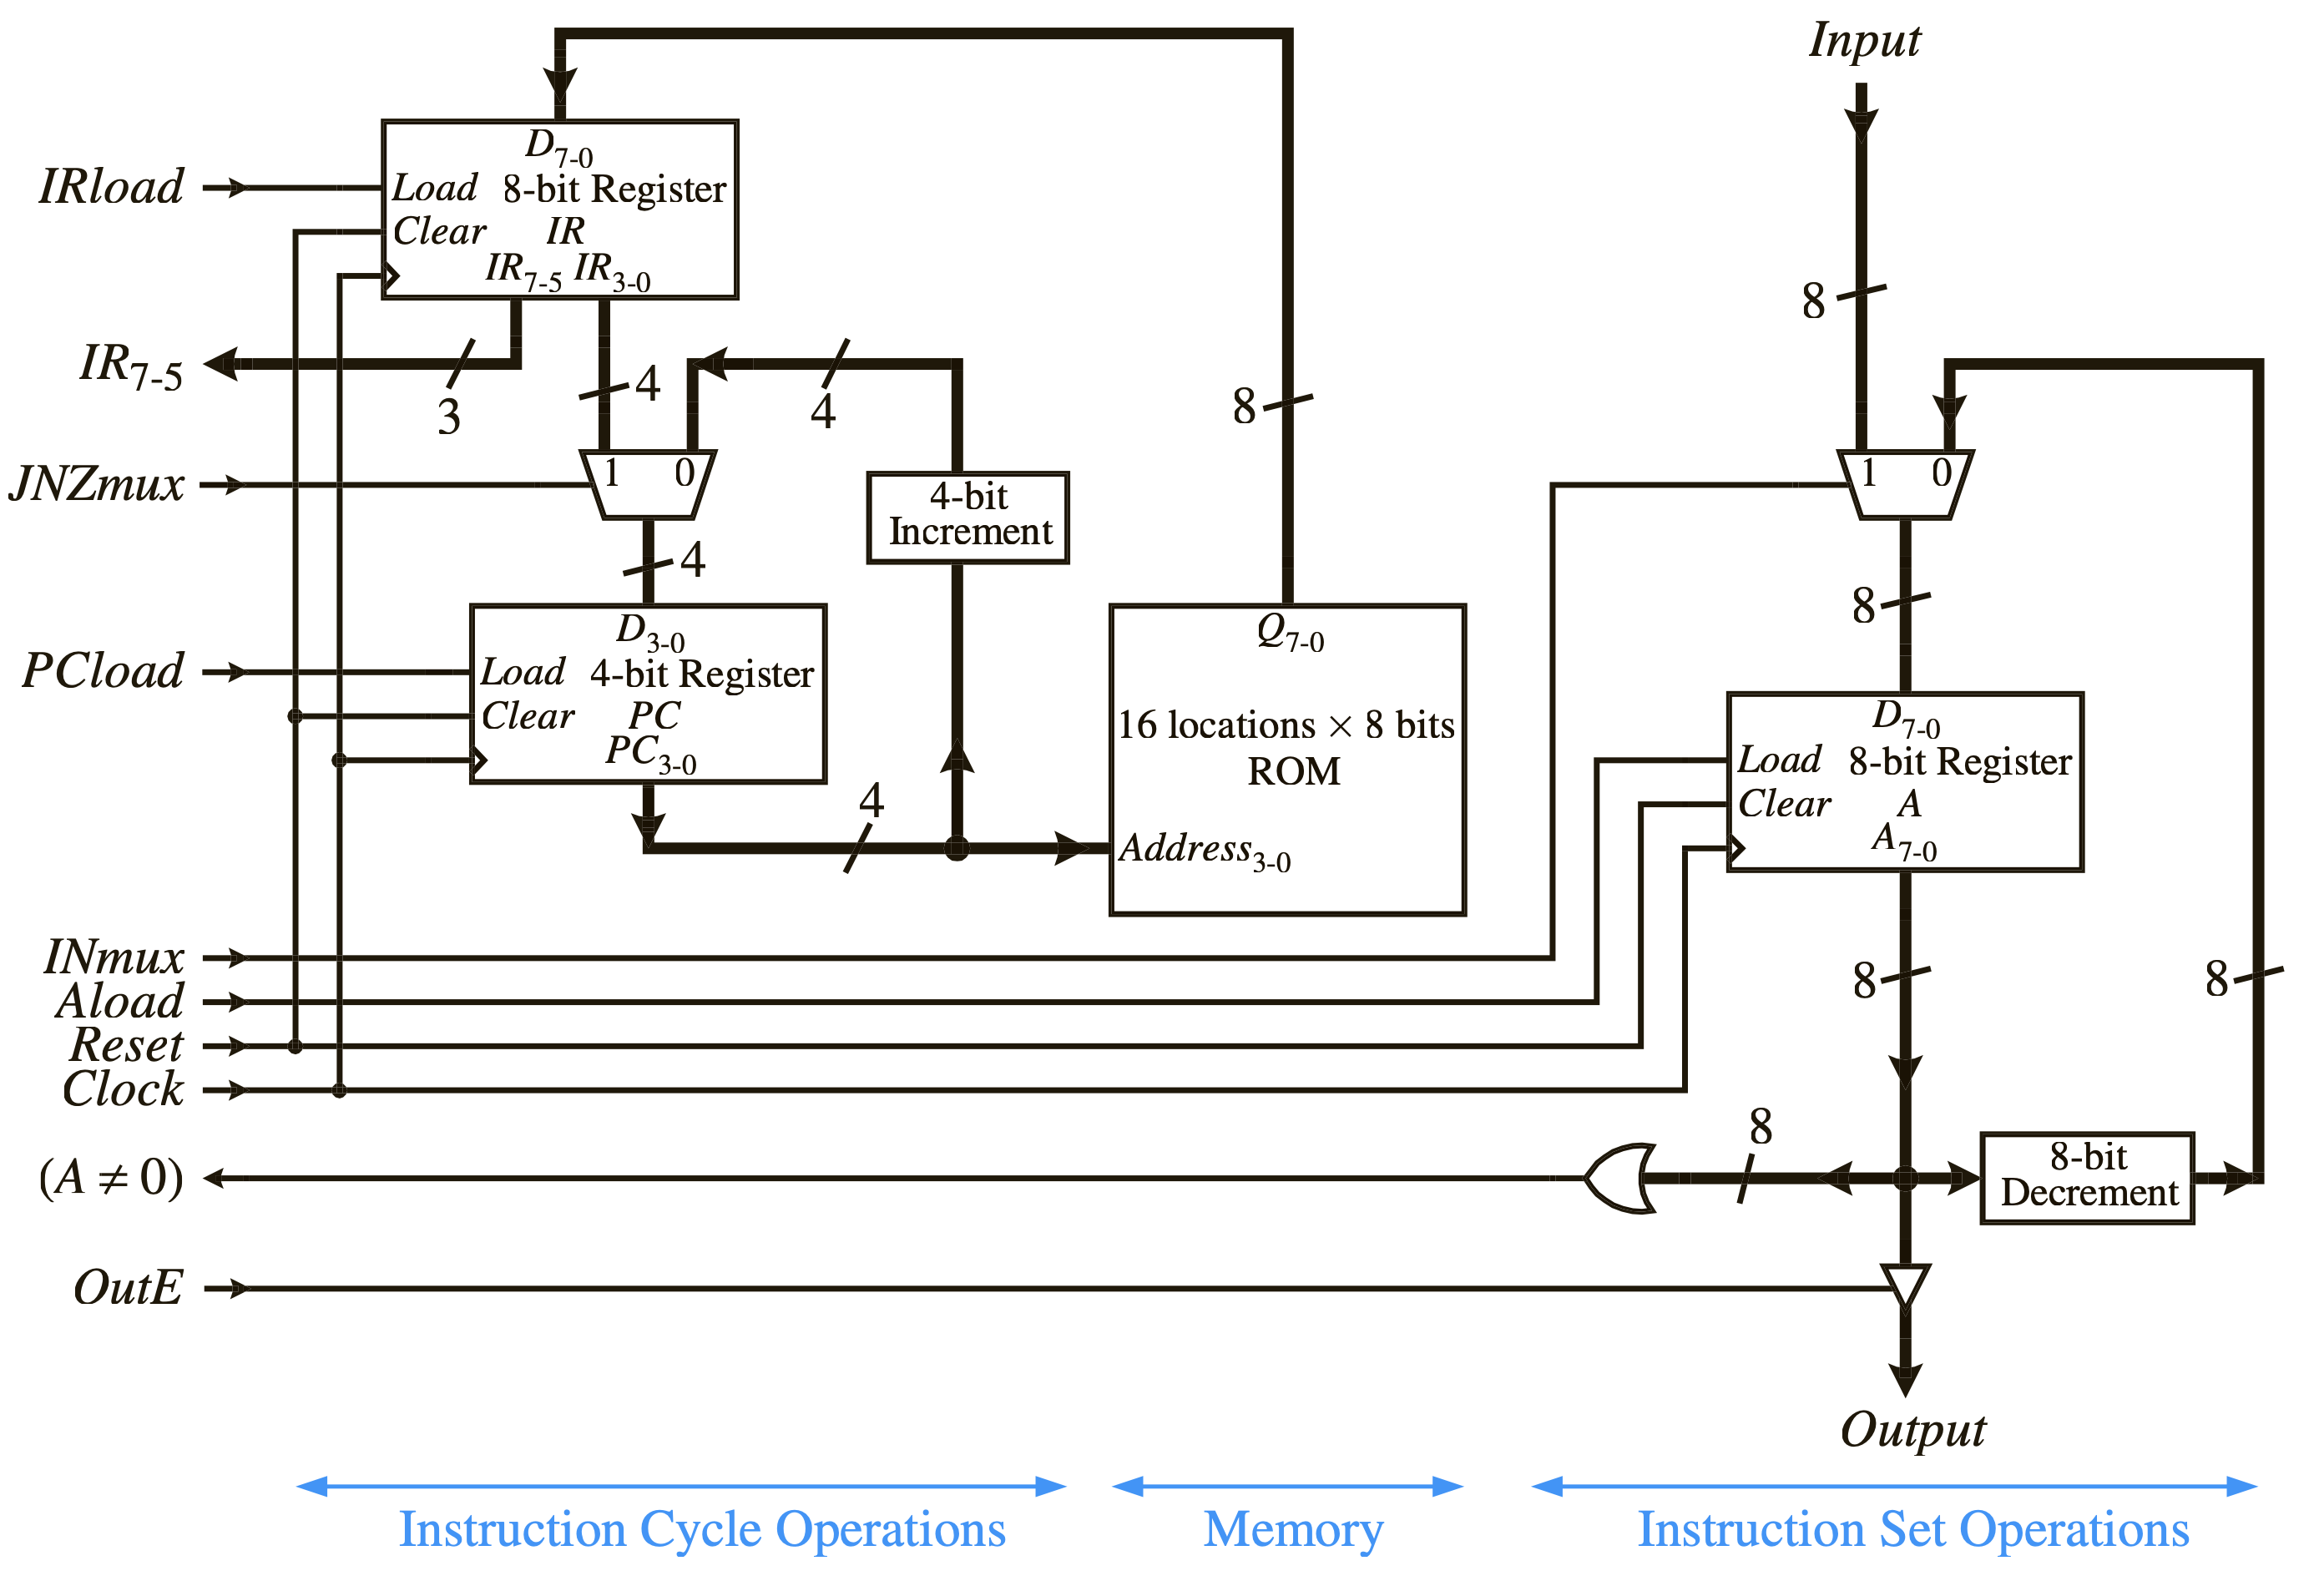
\includegraphics[width=\linewidth, height=415pt, keepaspectratio]{lect_10_ec1_datapath}
\caption{Datapath of the EC-1 microprocessor. Multiplexer inputs are numbered $1$ (left) and $0$ (right); a slash on a bus gives its width in bits. The clock and the reset are common to all registers, and the control signals (left) come from the control unit.}
\label{fig:ec1-dp}
\end{sidewaysfigure}

\subsection{ROM implementation}
FPGA vendors provide optimised memory blocks as \emph{IP cores} (intellectual-property modules). Using them guarantees that the memory is mapped to the FPGA's dedicated block-RAM resources rather than to general logic cells. In our implementation the program ROM is a one-port ROM generated by Intel's megafunction wizard (type \code{altsyncram}): an 8-bit wide, 32-word memory with a single clock and \emph{unregistered} output, initialised at programming time from a file in Intel HEX format. The memory is \emph{synchronous}: the address is sampled on the rising clock edge. As we shall see, this has consequences for the control unit.

\subsection{Intel HEX format}
\term{Intel HEX} is a text format that stores binary data for programming or initialising memories. Each line is a \emph{record} beginning with a colon: \texttt{:}\,\textit{LL}\,\textit{AAAA}\,\textit{TT}\,\textit{DD\dots DD}\,\textit{CC}, where \textit{LL} is the number of data bytes, \textit{AAAA} the starting address, \textit{TT} the record type (00 = data, 01 = end of file), \textit{DD} the data bytes and \textit{CC} a checksum chosen so that the sum of all bytes of the record is $00_{16}$ modulo 256. For example, the line
\begin{center}\ttfamily\small :100000006080A0C1E00000000000000000000000CF\end{center}
holds 16 (\texttt{10}$_{16}$) bytes starting at address 0000, the first five being the program of \cref{tab:ec1-prog}; its checksum is $\mathrm{CF}$ because $10+00+00+00+60+80+A0+C1+E0=331_{16}$ and $100_{16}-31_{16}=\mathrm{CF}_{16}$. The file is completed by a record for addresses 16--31 and the end-of-file record \texttt{:00000001FF}.

\subsection{Control unit}
The control unit is an FSM that carries out the instruction cycle, with one \textbf{fetch} state, one \textbf{decode} state and one execution state for each instruction (\cref{fig:ec1-fsm-nowait}).
\begin{description}[font=\sffamily\bfseries, leftmargin=1.2em]
  \item[FETCH (000)] Read the instruction at address PC into IR ($IR\leftarrow M[PC]$) and increment the PC ($PC\leftarrow PC+1$): $IRload=PCload=1$, $JNZmux=0$.
  \item[DECODE (001)] Examine the opcode $IR[7:5]$ and go to the execution state of the instruction (no control signals). Unused opcodes return to FETCH.
  \item[EXECUTE] \textbf{Input} (011): $A\leftarrow$ Input, $INmux=1$, $Aload=1$. \textbf{Output} (100): $OutE=1$. \textbf{Dec} (101): $A\leftarrow A-1$, $INmux=0$, $Aload=1$. \textbf{JNZ} (110): if $A\neq0$ then $PC\leftarrow IR[3:0]$ ($JNZmux=1$, $PCload=1$). \textbf{Halt} (111): stay here.
\end{description}
All execution states except Halt return to FETCH. The values of the control signals in each state are in \cref{tab:ec1-cs}.

\begin{table}[htbp]
\centering
\small
\caption{Control signals of the EC-1 in each state (``--'' = don't care).}
\label{tab:ec1-cs}
\begin{tabular}{lc|ccccccc}
\toprule
State & Code & IRload & PCload & INmux & Aload & JNZmux & OutE & Halt\\ \midrule
Fetch & 000 & 1 & 1 & -- & 0 & 0 & 0 & 0\\
Decode & 001 & 0 & 0 & -- & 0 & 0 & 0 & 0\\
Wait & 010 & 0 & 0 & -- & 0 & 0 & 0 & 0\\
Input & 011 & 0 & 0 & 1 & 1 & 0 & 0 & 0\\
Output & 100 & 0 & 0 & -- & 0 & 0 & 1 & 0\\
Decrement & 101 & 0 & 0 & 0 & 1 & 0 & 0 & 0\\
JumpNotZero & 110 & 0 & $(A\neq0)$ & -- & 0 & 1 & 0 & 0\\
Halt & 111 & 0 & 0 & -- & 0 & 0 & 0 & 1\\ \bottomrule
\end{tabular}
\end{table}

\subsubsection{The wait state}
The EC-1 uses a \emph{synchronous} ROM: it samples the address at the clock edge. In normal execution the PC is stable throughout the execution state, so the next fetch reads the right instruction. But when a jump is \emph{taken}, the PC is updated with the target address at the clock edge at the \emph{end} of the JNZ state. If the next state were FETCH, the ROM would sample the PC at the \emph{same edge} at which the PC changes, and may read the old address: a race condition. The solution is a \textbf{wait state}: JNZ goes to WAIT (010), a buffer cycle in which all control signals are idle, while the PC settles at the target; WAIT then goes to FETCH, in which the ROM safely samples the stable address (\cref{fig:ec1-fsm}). This is the same idea as the wait state of \cref{ex:cu2}.

\begin{figure}[htbp]
\centering
\begin{subfigure}[b]{396.7pt}\centering
  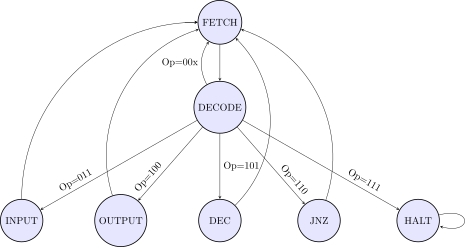
\includegraphics[width=394.7pt]{lect_10_ec1_fsm_no_wait}\caption{without wait state}\label{fig:ec1-fsm-nowait}
\end{subfigure}
\caption{State diagram of the EC-1 control unit.}
\end{figure}

\begin{figure}[htbp]
\centering
\ContinuedFloat
\begin{subfigure}[b]{396.7pt}\centering
  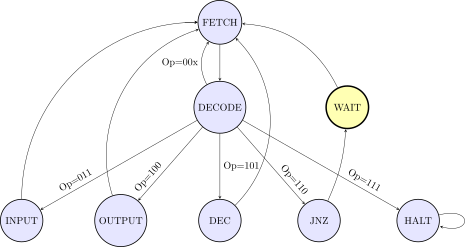
\includegraphics[width=394.7pt]{lect_10_ec1_fsm}\caption{with wait state}\label{fig:ec1-fsm}
\end{subfigure}
\caption[]{State diagram of the EC-1 control unit.}
\end{figure}

\subsubsection{State table and equations}
With the state codes of \cref{tab:ec1-cs}, and $O_2O_1O_0$ the opcode, the next-state equations follow from the state diagram:
\begin{align*}
 D_2 &= \mathrm{Decode}\cdot O_2 + \mathrm{Halt},\\
 D_1 &= \mathrm{Decode}\cdot O_1\cdot(O_2+O_0) + \mathrm{Halt} + \mathrm{JNZ},\\
 D_0 &= \mathrm{Fetch} + \mathrm{Decode}\cdot O_0\cdot(O_2+O_1) + \mathrm{Halt},
\end{align*}
where the state decoders are $\mathrm{Fetch}=Q_2'Q_1'Q_0'$, $\mathrm{Decode}=Q_2'Q_1'Q_0$, $\mathrm{Input}=Q_2'Q_1Q_0$, $\mathrm{Output}=Q_2Q_1'Q_0'$, $\mathrm{Dec}=Q_2Q_1'Q_0$, $\mathrm{JNZ}=Q_2Q_1Q_0'$ and $\mathrm{Halt}=Q_2Q_1Q_0$. Each term can be checked against \cref{fig:ec1-fsm}: for instance $D_1=1$ in the JNZ state because the next state is WAIT ($010$); in the decode state $D_1=1$ for the opcodes 011 (Input $=011$), 110 (JNZ $=110$) and 111 (Halt $=111$) but not 010 (unused, back to Fetch). WAIT and the other states return to $000$ by $D_2=D_1=D_0=0$. The outputs are
\begin{gather*}
 IRload = \mathrm{Fetch},\quad PCload = \mathrm{Fetch} + \mathrm{JNZ}\cdot(A\neq0),\quad INmux = \mathrm{Input},\\
 Aload = \mathrm{Input}+\mathrm{Dec},\quad JNZmux=\mathrm{JNZ},\quad OutE=\mathrm{Output},\quad Halt=\mathrm{Halt}.
\end{gather*}
\Cref{lst:ec1-cu} is the VHDL of the control unit; it is written directly from these equations (structural style), using three D flip-flops. \Cref{lst:ec1-dp} is the datapath. The components (flip-flops, registers, multiplexers, incrementer, decrementer, zero detector, three-state buffer) and the top level, which connects the two, are listed in \cref{app:listings}.

\vhdlfile{../vhdl/ec1_control_unit.vhd}{VHDL of the EC-1 control unit (structural, from the state equations).}{lst:ec1-cu}
\vhdlfile{../vhdl/ec1_datapath.vhd}{VHDL of the EC-1 datapath.}{lst:ec1-dp}

\subsection{Programming example: countdown from 10 to 1}
A program for EC-1 is a list of instruction bytes. \Cref{tab:ec1-prog} counts down from the input value to 1, outputting each value: \texttt{IN A} reads the starting value, \texttt{OUT A} displays $A$, \texttt{DEC A} decrements it, \texttt{JNZ 01} returns to \texttt{OUT A} while $A\neq0$, and \texttt{HALT} stops. Instructions are encoded by \cref{tab:ec1-is}; for example \texttt{JNZ 01} $=\texttt{110\,0\,0001}=\mathrm{C1}$.

\begin{table}[htbp]
\centering
\caption{EC-1 program: count down from the input value.}
\label{tab:ec1-prog}
\begin{tabular}{ccll}
\toprule Address & Hex & Assembly & Comment\\ \midrule
00 & 60 & \texttt{IN A} & input to $A$\\
01 & 80 & \texttt{OUT A} & output $A$\\
02 & A0 & \texttt{DEC A} & decrement $A$\\
03 & C1 & \texttt{JNZ 01} & jump to 01 if $A\ne0$\\
04 & E0 & \texttt{HALT} & done\\ \bottomrule
\end{tabular}
\end{table}

A testbench (similar to \cref{lst:tb}) generates a clock of period 10~ns, holds the reset for 20~ns, applies the input value 10 ($\bin{00001010}$) and runs until the \textit{halt} output is 1. \Cref{fig:ec1-sim} shows the result: the output counts $10,9,\dots,2,1$. For every value the processor goes through FETCH, DECODE and the execution state of \texttt{OUT A}, FETCH, DECODE, \texttt{DEC A}, FETCH, DECODE, \texttt{JNZ} and, when the jump is taken, WAIT; when $A$ reaches 0 the jump is not taken, PC advances to 04 and \texttt{HALT} is executed. The RTL viewer of Quartus shows the synthesised top level (\cref{fig:ec1-rtl}).

\begin{figure}[htbp]
\centering
{\small (a)~start: counting 10, 9, \dots}\\[3pt]
\wavestrip{lect_10_ec-1_count_10_9}{1}{175}
\wavestrip{lect_10_ec-1_count_10_9}{2}{175}
\wavestrip{lect_10_ec-1_count_10_9}{3}{175}
\caption{Simulation of the EC-1 running the countdown program (author's screenshots).}
\label{fig:ec1-sim}
\end{figure}

\begin{figure}[htbp]
\centering
\ContinuedFloat
\wavestrip{lect_10_ec-1_count_10_9}{4}{175}
\wavestrip{lect_10_ec-1_count_10_9}{5}{175}
\vspace{4pt}{\small (b)~end: \dots, 2, 1 and halt}\\[3pt]
\wavestrip{lect_10_ec-1_count_2_1}{1}{167}
\caption[]{Simulation of the EC-1 running the countdown program (author's screenshots).}
\end{figure}

\begin{figure}[htbp]
\centering
\ContinuedFloat
\wavestrip{lect_10_ec-1_count_2_1}{2}{167}
\wavestrip{lect_10_ec-1_count_2_1}{3}{167}
\wavestrip{lect_10_ec-1_count_2_1}{4}{167}
\caption[]{Simulation of the EC-1 running the countdown program (author's screenshots).}
\end{figure}

\begin{figure}[htbp]
\centering
\ContinuedFloat
\wavestrip{lect_10_ec-1_count_2_1}{5}{167}
\caption[]{Simulation of the EC-1 running the countdown program (author's screenshots).}
\end{figure}

\figw{\linewidth}{lect_10_rtl_viewer_ec-1}{RTL viewer (Quartus) of the top level of the EC-1: the control unit and the datapath (author's screenshot).}{fig:ec1-rtl}

\section{The EC-2 Microprocessor}\label{sec:ec2}
\subsection{Overview}
EC-2 improves on EC-1 in two ways: more instructions and a \emph{read/write} memory that stores both code and data. This is a \emph{stored-program computer} in the von Neumann sense (\cref{fig:vn-ec2}). EC-2 has
\begin{itemize}
  \item eight instructions;
  \item a $32\times8$-bit \textbf{RAM} that holds both the program and its variables (unified code/data memory);
  \item a \textbf{5-bit} address; and
  \item an adder/subtractor ALU.
\end{itemize}

\figw{191.1pt}{lect_10_von_neumann}{The von Neumann architecture: a single memory holds instructions and data, connected to the processor by a common bus.}{fig:vn-ec2}

\subsection{Instruction set}
\Cref{tab:ec2-is} lists the instructions. The three most significant bits are the opcode and the five least significant bits the memory address \texttt{aaaaa}. Memory operands make this a \emph{memory-reference} machine. \texttt{JZ} jumps if $A=0$ and \texttt{JPOS} if $A\ge0$ (a non-negative two's-complement value).

\begin{table}[htbp]
\centering
\caption{The EC-2 instruction set.}
\label{tab:ec2-is}
\begin{tabular}{llll}
\toprule
Mnemonic & Encoding & Operation & Description\\ \midrule
\texttt{LOAD A, addr} & \texttt{000 aaaaa} & $A\leftarrow M[aaaaa]$ & load $A$ from memory\\
\texttt{STORE A, addr} & \texttt{001 aaaaa} & $M[aaaaa]\leftarrow A$ & store $A$ to memory\\
\texttt{ADD A, addr} & \texttt{010 aaaaa} & $A\leftarrow A+M[aaaaa]$ & add memory to $A$\\
\texttt{SUB A, addr} & \texttt{011 aaaaa} & $A\leftarrow A-M[aaaaa]$ & subtract memory from $A$\\
\texttt{IN A} & \texttt{100 xxxxx} & $A\leftarrow$ Input & input to $A$\\
\texttt{JZ addr} & \texttt{101 aaaaa} & if $A=0$, $PC\leftarrow aaaaa$ & jump if zero\\
\texttt{JPOS addr} & \texttt{110 aaaaa} & if $A\ge0$, $PC\leftarrow aaaaa$ & jump if non-negative\\
\texttt{HALT} & \texttt{111 xxxxx} & halt & stop execution\\ \bottomrule
\end{tabular}
\end{table}

\subsection{Datapath}
The datapath (\cref{fig:ec2-dp}) is that of EC-1 with the following changes.
\begin{enumerate}
  \item A \textbf{5-bit address bus} to address 32 locations; the PC and IR address fields are 5 bits wide.
  \item A \textbf{RAM} instead of the ROM, so that \texttt{STORE} is possible.
  \item A \textbf{memory-address multiplexer} (\textit{MemInst}): during \emph{fetch} the address comes from the PC ($0$); during the execution of LOAD, STORE, ADD and SUB it comes from $IR[4:0]$ ($1$). This shared address bus is the fundamental constraint of the von Neumann design.
  \item An \textbf{ALU} that adds ($\mathit{Sub}=0$) or subtracts ($\mathit{Sub}=1$) the RAM output from $A$.
  \item A \textbf{4-to-1 accumulator multiplexer} (\textit{Asel}) that selects the input of $A$: the RAM output (LOAD, $00$), the ALU output (ADD, SUB, $01$) or the input port (IN, $10$); code $11$ selects the constant 0.
  \item Flag detectors for $A=0$ (\textit{Zero}, an 8-input NOR gate) and $A\ge0$ (\textit{Pos}, the inverted sign bit $A_7$), the status signals for JZ and JPOS.
\end{enumerate}
The control signals are \textit{IRload}, \textit{PCload}, \textit{MemInst}, \textit{MemWr} (RAM write enable), \textit{Asel}, \textit{Aload}, \textit{Sub}, \textit{JMPmux} (selects the jump address as the new PC) and \textit{Halt}.

\begin{sidewaysfigure}[p]
\centering
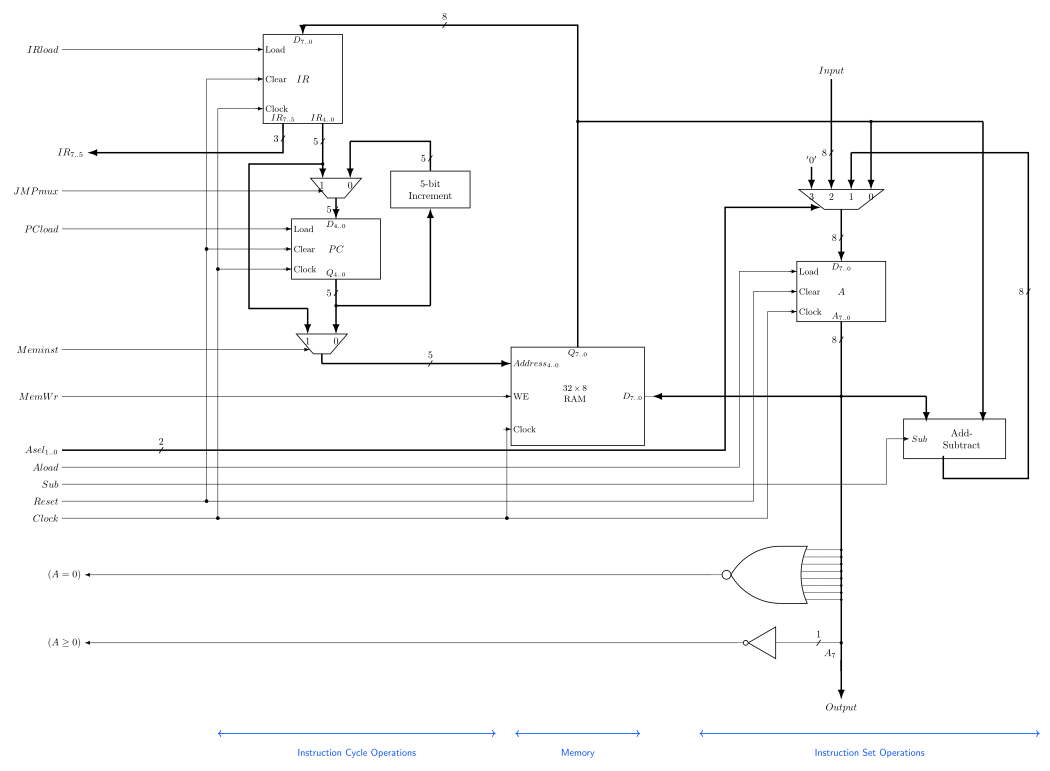
\includegraphics[width=\linewidth, height=425pt, keepaspectratio]{lect_10_ec2_datapath}
\caption{Datapath of the EC-2 microprocessor. The memory-address multiplexer \textit{MemInst} selects the PC (0) in the fetch state and the address field of the IR (1) when a memory operand is accessed; the accumulator multiplexer is selected by $Asel_{1..0}$ ($00$ RAM, $01$ ALU, $10$ input port, $11$ constant $0$). $(A=0)$ and $(A\ge0)$ are the status signals for \texttt{JZ} and \texttt{JPOS}.}
\label{fig:ec2-dp}
\end{sidewaysfigure}

\subsection{Control unit}
The instruction cycle now includes memory access (\cref{tab:ec2-cs}). In \textbf{fetch} ($\mathit{MemInst}=0$) the instruction is read from the address in the PC into IR and the PC is incremented. In \textbf{decode} the opcode selects the execution state. In \textbf{execute}: \texttt{LOAD} sets $MemInst=1$, reads the RAM and loads $A$; \texttt{STORE} sets $MemInst=1$ and $MemWr=1$, writing $A$ into the RAM; \texttt{ADD} and \texttt{SUB} set $MemInst=1$, read the RAM and load $A$ with the ALU result; \texttt{IN} loads $A$ from the input port; \texttt{JZ} and \texttt{JPOS} load the PC with the address field if the flag $Z$ or $P$ is true; \texttt{HALT} stops. The FSM is \cref{fig:ec2-fsm}, with ten states coded in 4 bits.

\begin{table}[htbp]
\centering
\scriptsize
\caption{Control signals of the EC-2 in each state ($Z$: $A=0$; $P$: $A\ge0$).}
\label{tab:ec2-cs}
\setlength{\tabcolsep}{3.5pt}
\begin{tabular}{lc|cccccccccc}
\toprule
State & Code & IRload & PCload & MemInst & MemWr & Asel & Aload & Sub & JMPmux & Halt\\ \midrule
Fetch & 0000 & 1 & 1 & 0 & 0 & -- & 0 & 0 & 0 & 0\\
Decode & 0001 & 0 & 0 & 0 & 0 & -- & 0 & 0 & 0 & 0\\
Load & 0010 & 0 & 0 & 1 & 0 & 00 & 1 & 0 & 0 & 0\\
Store & 0011 & 0 & 0 & 1 & 1 & -- & 0 & 0 & 0 & 0\\
Add & 0100 & 0 & 0 & 1 & 0 & 01 & 1 & 0 & 0 & 0\\
Sub & 0101 & 0 & 0 & 1 & 0 & 01 & 1 & 1 & 0 & 0\\
In & 0110 & 0 & 0 & 0 & 0 & 10 & 1 & 0 & 0 & 0\\
Jz & 0111 & 0 & $Z$ & 0 & 0 & -- & 0 & 0 & 1 & 0\\
Jpos & 1000 & 0 & $P$ & 0 & 0 & -- & 0 & 0 & 1 & 0\\
Halt & 1001 & 0 & 0 & 0 & 0 & -- & 0 & 0 & 0 & 1\\ \bottomrule
\end{tabular}
\end{table}

\begin{figure}[htbp]
\centering
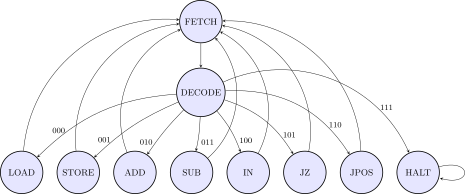
\includegraphics[max width=0.9\linewidth, max height=9cm]{lect_10_ec2_fsm}
\caption{State diagram of the EC-2 control unit.}
\label{fig:ec2-fsm}
\end{figure}

With the state codes of \cref{tab:ec2-cs}, and the opcode $O_2O_1O_0$ examined in the decode state, the next-state equations are
\begin{align*}
 D_3 &= \mathrm{Decode}\cdot O_2O_1 + \mathrm{Halt}, & D_2 &= \mathrm{Decode}\cdot(O_2\xor O_1),\\
 D_1 &= \mathrm{Decode}\cdot O_1', & D_0 &= \mathrm{Fetch} + \mathrm{Decode}\cdot O_0 + \mathrm{Halt},
\end{align*}
and the outputs are
\begin{gather*}
 IRload=\mathrm{Fetch},\quad PCload=\mathrm{Fetch}+\mathrm{Jz}\cdot Z+\mathrm{Jpos}\cdot P,\quad JMPmux=\mathrm{Jz}+\mathrm{Jpos},\\
 MemInst=\mathrm{Load}+\mathrm{Store}+\mathrm{Add}+\mathrm{Sub},\quad MemWr=\mathrm{Store},\\
 Asel_1=\mathrm{In},\quad Asel_0=\mathrm{Add}+\mathrm{Sub},\quad Aload=\mathrm{Load}+\mathrm{Add}+\mathrm{Sub}+\mathrm{In},\quad Sub=\mathrm{Sub},\quad Halt=\mathrm{Halt}.
\end{gather*}
As a check of $D_2$: Add ($010\to0100$), Sub ($011\to0101$), In ($100\to0110$) and Jz ($101\to0111$) have $O_2\xor O_1=1$; Load, Store and Halt/Jpos ($11x$) have $O_2\xor O_1=0$ and $D_2=0$. The complete VHDL of the control unit, the datapath, the components (including the RAM with its initial contents) and the top level is in \cref{app:listings}.

\subsection{Memory wait states and timing}
EC-2 is a \emph{multi-cycle} processor: every instruction takes several clock cycles, and some states act as wait states for the memory (\cref{fig:ec2-wait}). The whole \textbf{fetch} cycle is a wait for the instruction to be read. The execution states of the memory-reading instructions (\texttt{LOAD}, \texttt{ADD}, \texttt{SUB}) drive the address bus and wait for the RAM data, which is captured in $A$ at the end of the cycle (asynchronous read). A \texttt{STORE} sets up the address and data and asserts \textit{MemWr}, and the RAM writes on the clock edge (synchronous write). Waiting for one cycle guarantees that the signals are stable through the chain address multiplexer $\to$ RAM $\to$ data out.

\figw{250.3pt}{lect_10_ec2_wait_state}{Multi-cycle memory access in the EC-2.}{fig:ec2-wait}

\subsection{Programming example: GCD}
The program of \cref{tab:ec2-gcd} implements Euclid's algorithm of \cref{ex:gcd}: \texttt{while (X != Y) \{ if (X > Y) X -= Y; else Y -= X; \}}. The variables occupy memory locations 30 ($X$) and 31 ($Y$), which are initialised to 15 and 25. Because EC-2 has only \texttt{JZ} and \texttt{JPOS}, the compare is done by subtraction: $A=X-Y$ is zero if they are equal (jump to the end) and positive if $X>Y$; a \texttt{JPOS} after a result that is known to be positive acts as an unconditional jump.

\begin{table}[htbp]
\centering
\caption{EC-2 program that computes the GCD of the numbers in locations 30 and 31 (addresses in decimal).}
\label{tab:ec2-gcd}
\begin{tabular}{ccll}
\toprule Address & Hex & Assembly & Comment\\ \midrule
00 & 1E & \texttt{LOAD A, 30} & load $X$\\
01 & 7F & \texttt{SUB A, 31} & $A=X-Y$\\
02 & AA & \texttt{JZ 10} & if $X=Y$, done\\
03 & C8 & \texttt{JPOS 08} & if $X>Y$, update $X$\\
04 & 1F & \texttt{LOAD A, 31} & else ($X<Y$) load $Y$\\
05 & 7E & \texttt{SUB A, 30} & $A=Y-X$\\
06 & 3F & \texttt{STORE A, 31} & save new $Y$\\
07 & C0 & \texttt{JPOS 00} & loop\\
08 & 3E & \texttt{STORE A, 30} & save new $X$\\
09 & C0 & \texttt{JPOS 00} & loop\\
10 & E0 & \texttt{HALT} & result in $M[30]$\\ \bottomrule
\end{tabular}
\end{table}

\paragraph{Trace.} Starting with $X=15$, $Y=25$: $A=X-Y=-10$; \texttt{JZ} and \texttt{JPOS} do not jump; $A\leftarrow Y=25$, $A\leftarrow A-X=10$, $Y\leftarrow10$ and the program loops. Now $A=15-10=5>0$: \texttt{JPOS 08}; $X\leftarrow5$; loop. Then $A=5-10=-5$: $A\leftarrow10$, $A\leftarrow5$, $Y\leftarrow5$; loop. Now $A=5-5=0$ and \texttt{JZ 10} jumps to \texttt{HALT}; $M[30]=5$, the GCD of 15 and 25. \Cref{fig:ec2-sim} shows the simulation of the processor running this program, \cref{fig:ec2-rtl} the synthesised top level.

\begin{figure}[htbp]
\centering
{\small (a)}\\[2pt]
\wavestrip{lect_10_ec2_sim_1}{1}{130}
\wavestrip{lect_10_ec2_sim_1}{2}{130}
\wavestrip{lect_10_ec2_sim_1}{3}{130}
\wavestrip{lect_10_ec2_sim_1}{4}{130}
\caption{Simulation of the EC-2 computing the GCD of 25 and 15: (a)--(d)~successive parts of the run: $Y$ becomes 10, then $X$ becomes 5, then $Y$ becomes 5, and finally $A=X-Y=0$, \texttt{JZ} is taken and the processor halts. Author's screenshots.}
\label{fig:ec2-sim}
\end{figure}

\begin{figure}[htbp]
\centering
\ContinuedFloat
\wavestrip{lect_10_ec2_sim_1}{5}{130}
{\small (b)}\\[2pt]
\wavestrip{lect_10_ec2_sim_2}{1}{130}
\wavestrip{lect_10_ec2_sim_2}{2}{130}
\wavestrip{lect_10_ec2_sim_2}{3}{130}
\caption[]{Simulation of the EC-2 computing the GCD of 25 and 15}
\end{figure}

\begin{figure}[htbp]
\centering
\ContinuedFloat
\wavestrip{lect_10_ec2_sim_2}{4}{130}
\wavestrip{lect_10_ec2_sim_2}{5}{130}
{\small (c)}\\[2pt]
\wavestrip{lect_10_ec2_sim_3}{1}{130}
\wavestrip{lect_10_ec2_sim_3}{2}{130}
\caption[]{Simulation of the EC-2 computing the GCD of 25 and 15}
\end{figure}

\begin{figure}[htbp]
\centering
\ContinuedFloat
\wavestrip{lect_10_ec2_sim_3}{3}{130}
\wavestrip{lect_10_ec2_sim_3}{4}{130}
\wavestrip{lect_10_ec2_sim_3}{5}{130}
{\small (d)}\\[2pt]
\wavestrip{lect_10_ec2_sim_4}{1}{130}
\caption[]{Simulation of the EC-2 computing the GCD of 25 and 15}
\end{figure}

\begin{figure}[htbp]
\centering
\ContinuedFloat
\wavestrip{lect_10_ec2_sim_4}{2}{130}
\wavestrip{lect_10_ec2_sim_4}{3}{130}
\wavestrip{lect_10_ec2_sim_4}{4}{130}
\wavestrip{lect_10_ec2_sim_4}{5}{130}
\caption[]{Simulation of the EC-2 computing the GCD of 25 and 15}
\end{figure}

\figw{\linewidth}{lect_10_rtl_viewer_ec2}{RTL viewer (Quartus) of the EC-2 top level (author's screenshot).}{fig:ec2-rtl}

\subsection{Program loading and self-modifying code}
In \cref{lst:ec2-ram} (Appendix) the program is hard-coded into the RAM initial contents. A real system loads programs from storage into RAM using a \term{bootloader}, a small program that is already in memory. EC-2 has no \emph{indirect addressing} (no way to address memory through a pointer), so the loader cannot write to \texttt{RAM[i]} with a variable $i$. The solution exploits the von Neumann property that \emph{code is data}: the program \textbf{modifies its own} \texttt{STORE} instruction to change its destination (\cref{tab:boot}):
\begin{enumerate}
  \item read a byte from the input;
  \item store it at the target address (the address field of the \texttt{STORE} at location 01);
  \item read the \texttt{STORE} instruction itself (\texttt{LOAD A, 01}), add 1 (the constant at location 06) to its address field, and write it back: \texttt{STORE A,10} becomes \texttt{STORE A,11};
  \item loop to read the next byte.
\end{enumerate}

\begin{table}[htbp]
\centering
\caption{A bootloader for the EC-2 using self-modifying code; the loaded program starts at address 10.}
\label{tab:boot}
\begin{tabular}{cll}
\toprule Address & Assembly & Comment\\ \midrule
00 & \texttt{IN A} & read a byte from storage\\
01 & \texttt{STORE A, 10} & write to address 10 (the target) -- \emph{this instruction is modified}\\
02 & \texttt{LOAD A, 01} & load the instruction at 01\\
03 & \texttt{ADD A, 06} & add 1 to the address field (constant at 06)\\
04 & \texttt{STORE A, 01} & save the modified instruction (\texttt{STORE A,11})\\
05 & \texttt{JPOS 00} & loop for the next byte\\
06 & \texttt{01} & the constant 1\\
10 & xx & start of the destination of the loaded program\\ \bottomrule
\end{tabular}
\end{table}

\begin{caution}[Self-modifying code]
The same property that makes a stored-program computer powerful also makes it vulnerable: a program that can change its own instructions, or data that can be executed as instructions, is a source of bugs and of security attacks. Modern processors separate executable from writable memory.
\end{caution}

\section{EC-1 versus EC-2}
\Cref{tab:ec1-ec2} summarises the architectural step from a small accumulator machine with a program ROM to a stored-program computer.

\begin{table}[htbp]
\centering
\small
\caption{Comparison of EC-1 and EC-2.}
\label{tab:ec1-ec2}
\begin{tabularx}{\linewidth}{@{}lXX@{}}
\toprule
Feature & EC-1 & EC-2\\ \midrule
Architecture & Hardwired control, accumulator machine with a program ROM & Von Neumann: unified memory for code and data\\
Memory & $16\times8$ ROM (program only); no data memory & $32\times8$ RAM (code and data)\\
Instruction set & 5 instructions (input, output, decrement, conditional jump, halt) & 8 instructions (load/store, add/subtract, input, conditional jumps, halt)\\
Addressing & 4-bit program address; operand is the accumulator & 5-bit direct memory addressing\\
Control unit & Fetch--decode--execute with one wait state (jump) & Multi-state memory access with wait cycles\\
Program can modify itself & no & yes (code in RAM)\\ \bottomrule
\end{tabularx}
\end{table}

\begin{chaptersummary}
\begin{itemize}
  \item A \textbf{general-purpose processor} is a dedicated processor whose task is to \textbf{fetch, decode and execute} stored instructions. Its design consists of the \textbf{instruction set}, the \textbf{datapath} and the \textbf{control unit}.
  \item \textbf{EC-1}: 8-bit accumulator machine, 5 instructions, 16-word ROM. The control unit has FETCH, DECODE and execution states; a \textbf{wait state} after JNZ prevents a race with the synchronous ROM.
  \item Programs are loaded into memory with an \textbf{Intel HEX} file; each record has a byte count, address, type, data and checksum.
  \item \textbf{EC-2}: 8 instructions, $32\times8$ RAM for code and data, ALU, flags, and multi-cycle memory access. The memory-address multiplexer shares one address bus between instruction fetch and data access.
  \item With the code in RAM the processor becomes a \textbf{von Neumann} computer: programs can be loaded by a bootloader and can modify themselves.
  \item The processor is an \textbf{interpreter}: the FSM translates opcodes into control signals. Flexibility costs control-unit complexity.
\end{itemize}
\end{chaptersummary}

\chapsec{Exercises}
\begin{exlist}
  \item \textbf{Ramp generator (EC-1).} Write an EC-1 program that outputs a value counting down from the input $n$ to \emph{0} (a descending ramp, as would be sent to a digital-to-analogue converter to generate a sawtooth). Show the waveform simulation. (\emph{Hint:} \cref{tab:ec1-prog} outputs $n,\dots,1$.) Why can the EC-1 not repeat the ramp forever, and what instruction would it need?
  \item \textbf{Odd/even detector (EC-1).} Determine whether the input number is odd or even. The program may not test bit 0 directly. \emph{Hint:} ``ping-pong'' between two decrement points: subtract 1, test, subtract 1, test; the \texttt{HALT} at which the program stops tells the parity. Write the program, encode it in hexadecimal and trace it for the inputs 5 and 6.
  \item \textbf{Multiplication (EC-2).} Compute the product of the numbers in $M[30]$ and $M[31]$ by repeated addition: $Sum=0$; loop: add $A$ to $Sum$, decrement $B$; stop when $B=0$. Write the program, using constants in memory, and trace it for $3\times4$. (EC-2 has no decrement instruction: use \texttt{SUB} with a memory location containing 1.)
  \item \textbf{Absolute difference (EC-2).} Compute $|A-B|$ for the numbers in $M[30]$, $M[31]$ and store it in $M[31]$.
  \item Encode in hexadecimal: (a)~EC-1: \texttt{IN A}, \texttt{DEC A}, \texttt{DEC A}, \texttt{OUT A}, \texttt{HALT}; (b)~EC-2: \texttt{LOAD A,5}, \texttt{ADD A,6}, \texttt{STORE A,7}, \texttt{HALT}.
  \item Write the Intel HEX record for the 5-byte EC-1 program \texttt{60 80 A0 C1 E0} at address 0000, compute its checksum, and give the end-of-file record.
  \item Trace the EC-1 program of \cref{tab:ec1-prog} for the input 2: list for each clock cycle the state, PC, IR, $A$ and output.
  \item Explain what would go wrong in the EC-1 if the wait state after JNZ were removed and the ROM were a synchronous ROM, with a timing sketch of PC, the ROM address sampling and the instruction register.
  \item Why does the EC-2 need the \textit{MemInst} multiplexer? What would be the consequence of using two separate memories for instructions and data (the Harvard architecture)?
  \item How many clock cycles does the EC-2 need to execute \texttt{LOAD A,30}, \texttt{SUB A,31} and \texttt{HALT}? (Use the state diagram: fetch, decode and execute each take one cycle.)
  \item Extend the EC-1 with a new instruction \texttt{INC A} (opcode 010). Which changes are needed in the datapath, in the state diagram and in the next-state and output equations?
  \item Add a \texttt{JMP addr} (unconditional jump) to EC-2 using the unused states. Which parts of the design change?
  \item Compute the contents of $M[30]$ when the EC-2 GCD program is run with $X=48$, $Y=18$, and the number of times that \texttt{SUB} is executed.
\end{exlist}

\chapsec{Further Reading}
The idea of building a processor from a datapath and an FSM, and the EC-1 and EC-2 designs on which this chapter is based, are described in Hwang~\cite{hwang2005,hwang2018}. For modern microarchitecture, Harris and Harris~\cite{harris2012} develop a complete MIPS processor in the same style (single-cycle, multi-cycle and pipelined). The stored-program concept was first described by von Neumann~\cite{vonneumann1945}.
